% Kapitel 2 mit den entsprechenden Unterkapiteln
% Die Unterkapitel können auch in separaten Dateien stehen,
% die dann mit dem \include-Befehl eingebunden werden.
%-------------------------------------------------------------------------------
\chapter{Analyse der Produktfunktionen}

Dieser Abschnitt stellt die Basis für die Festlegung der Architektur dar. Die
Festlegung einer geeigneten Architektur geschieht aufgrund der im Pflichtenheft
analysierten Produktfunktionen und nicht-funktionalen Anforderungen, die
realisiert werden müssen. Jede betrachtete Funktion wird in einem eigenen
Unterkapitel dokumentiert.  Fügen Sie bitte so viele Unterkapitel ein, wie
Produktfunktionen im Pflichtenheft vorhanden sind. Auch die nicht-funktionalen
Anforderungen sind so weit möglich entsprechend darzustellen.

%Die Kapitel müssen mit Inhalt gefüllt werden!. Eine Bereiche habe ich beuwsst schon bei der Verteildung der Diagramme zusammengefasst 
%In diesen Bereichen möchte ich euch bitten die jeweiligen Unterpunkte kurz mit den Oberpunkten zu vergleichen und zu argumentieren 
%warum es sich um triviale Spezialfälle handelt die keiner näheren beschreibung bedürfen
%
% Ich hab mal immer davon geschrieben welche Bereich von wem gemacht werden





%Christian/Matthias
\section{Analyse von Funktionalität :  Renderloop}
Da es sich um ein System handelt, indem eine ständige Berechnung (Loop) zur Laufzeit notwendig wird, einerseits durch die 3D-Anzeige die eine ständige aktualisierung erwartet und andererseits durch
die Simulation an sich, ist es sinnig diesen Vorgang ebenfalls näher zu beleuchten.
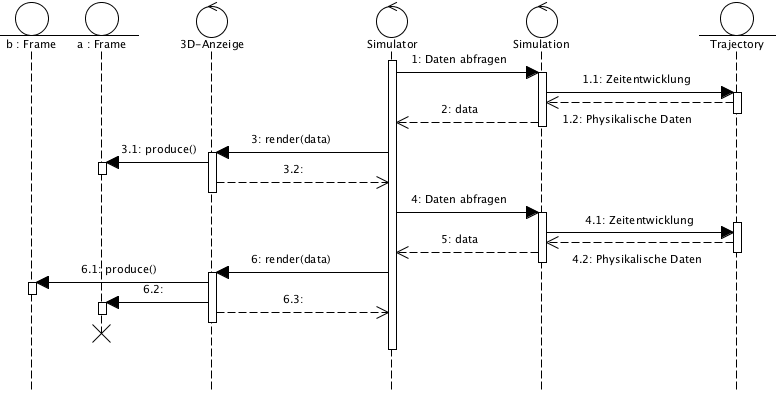
\includegraphics[width=10cm]{bilder/render_loop}

%Marco:
\section{Analyse von Funktionalität /F100/ :  Spezifikation einlesen }
%Simon:
\section{Analyse von Funktionalität /F200/ :  Starten/Stoppen der Simulation}
%Robin
\section{Analyse von Funktionalität /F300/ :  Pausieren der Simulation}
%Daniel
\section{Analyse von Funktionalität /F400o/ :  Video aufzeichnen}
Der Anwender kann über die GUI die Eingabe tätigen ein Video aufzeichnen zu wollen, sofern nicht gerade eine Aufnahme läuft. Die GUI gibt diese Anweisung an die 3D-Anzeige weiter, die nun mit der
Videoaufnahme beginnt. Dies geschieht so lange, bis der Anwender die Videoaufzeichnung stoppt. In diesem Fall wird die Aufzeichnung angehalten und die Videodatei wird gespeichert.
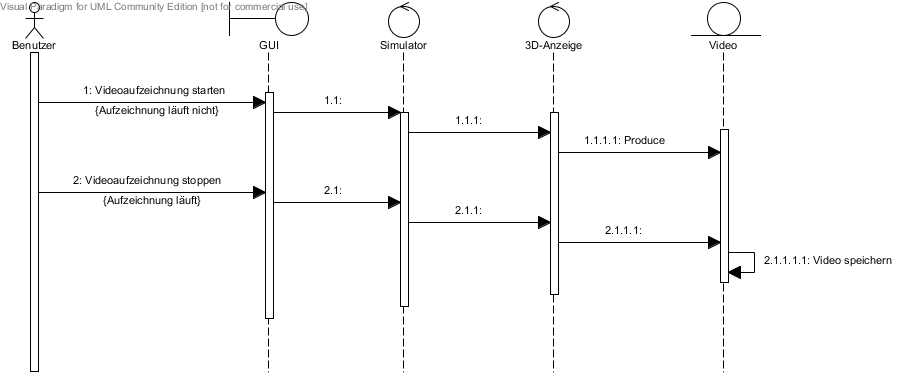
\includegraphics[width=16cm]{bilder/Video_aufzeichnen}
%Matthias/Christian
\section{Analyse von Funktionalität /F500/ :  Einstellungen ändern}
\section{Analyse von Funktionalität /F510o/ :  Physikalische Paramter anpassen}
\subsection{Analyse von Funktionalität /F511o/ :  Gravitation anpassen}
\subsection{Analyse von Funktionalität /F512o/ :  Wagenmasse anpassen}
\subsection{Analyse von Funktionalität /F520/ :  Simulationsparameter ändern}
%Matthias
\subsection{Analyse von Funktionalität /F521o/ :  Dekorative Umgebung anpassen}
\subsection{Analyse von Funktionalität /F522o/ :  Simulatioszeit anpassen}
%Matthias
\subsection{Analyse von Funktionalität /F530/ :  Graphische Einstellungen ändern}
%Daniel
\subsection{Analyse von Funktionalität /F531/ :   Neuanordnung (Interface)}
Der Anwender hat die Möglichkeit die Segmente innerhalb der GUI nach seinen eigenen Bedürfnissen einzurichten. Um dies zu tun, muss er nur die Eingabe in der GUI tätigen, die Segmente entsperren zu wollen.
Nun sind sie so lange frei positionierbar, bis er die Eingabe tätigt sie wieder sperren zu wollen.
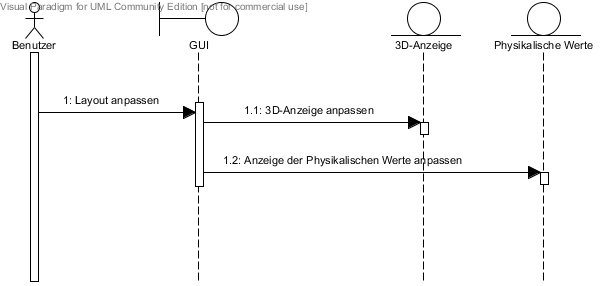
\includegraphics[width=16cm]{bilder/Interface_Neuanordnung}
%Simon
\subsection{Analyse von Funktionalität /F532/ :  Ein-/Ausblenden von Beschleunigungsdaten}
%Robin
\subsection{Analyse von Funktionalität /F533o/ :  Kameraperspektive ändern}
%Konstantin
\section{Analyse von Funktionalität /F1000/ :  Warnung vor hoher Beschleunigung}
%Marco:
\section{Analyse von Funktionalität /F1100/ :  Erkennung von Veränderungen an der Ursprungsdatei}